\documentclass[10pt]{article}

\usepackage{amssymb}
\usepackage[margin=1in,bmargin=1in,top=1in]{geometry}
\usepackage[charter]{mathdesign}
\usepackage{amsmath,esint}
\usepackage{mathtools}
\usepackage{float}
\usepackage[T1]{fontenc}
\usepackage{graphicx}
\usepackage{subfig}
\usepackage{fancyhdr, graphicx, kantlipsum, lipsum}
\usepackage{titling}
\usepackage[english]{babel}
\usepackage[utf8]{inputenc}
\usepackage{abstract}
\usepackage{wrapfig}
\usepackage{indentfirst}
\usepackage{textcomp}
\usepackage{url}
\usepackage[toc,page]{appendix}
\usepackage{listings}
\usepackage[style=numeric-comp,backend=biber]{biblatex}
\usepackage{csquotes}
\usepackage{gensymb}
\usepackage{pdfpages}
\usepackage{hyperref}
\usepackage{booktabs}
\usepackage[labelfont=bf]{caption}
\usepackage{siunitx}
\usepackage{longtable}
\usepackage{perpage}
\usepackage{scrextend}
\usepackage{etoolbox}
\usepackage{ragged2e}
\usepackage[intoc]{nomencl}
\usepackage{tikz}
\usepackage{adjustbox}
\usepackage[bottom]{footmisc}
\usepackage{bookmark}
\usepackage{setspace}
\usepackage{color}
\usepackage[version=4]{mhchem}
\usepackage{tabularx}
\usepackage{pgfplots} %http://www.ctan.org/pkg/pgfplots
\usepackage{pseudocode}
\usetikzlibrary{patterns}

\hypersetup{
	colorlinks=true,
	linkcolor=blue,
	filecolor=magenta,      
	urlcolor=cyan,
	citecolor=blue,
	bookmarksopen=true
}

% URL formatting
\urlstyle{same}
\def\UrlBreaks{\do\/\do-}

% Table Caption formatting
\captionsetup[table]{labelsep=space,skip=2pt,justification=raggedright,singlelinecheck=false}
\captionsetup[figure]{font={stretch=1}}
\sisetup{table-number-alignment=center}

% Miscellaneous formatting
\frenchspacing
\pagestyle{fancy}
\addbibresource{Bibliography.bib}
\DeclareNameAlias{default}{last-first}
\numberwithin{table}{section}
\numberwithin{figure}{section}
\numberwithin{equation}{section}
\MakePerPage{footnote}
\setlength\heavyrulewidth{0.25ex}
\definecolor{mygreen}{RGB}{28,172,0} % color values Red, Green, Blue
\definecolor{mylilas}{RGB}{170,55,241}
\bookmarksetup{open,numbered}


%Header/Footer formatting
\renewcommand{\headrulewidth}{0pt}
\renewcommand{\footrulewidth}{0pt}
\fancyhf{}
\fancyhead{}

% Additional commands
\makeatletter
\def\tagform@#1{\maketag@@@{[#1]\@@italiccorr}}
\makeatother
\makeatletter
\newcommand*{\rom}[1]{\expandafter\@slowromancap\romannumeral #1@}
\makeatother
\newcolumntype{C}[1]{>{\centering\let\newline\\\arraybackslash}b{#1}}
\DeclareUnicodeCharacter{0301}{}


%%%%%%%%%%%%%%%%%%%%%%%%%%%%%%%%%%%%%
%			Commands to draw the manipulator			%
%%%%%%%%%%%%%%%%%%%%%%%%%%%%%%%%%%%%%
\newcommand{\nvar}[2]{%
	\newlength{#1}
	\setlength{#1}{#2}
}


\nvar{\dg}{0.3cm}
\def\dw{0.25}\def\dh{0.5}
\nvar{\ddx}{1.5cm}


\def\link{\draw [double distance=1.5mm, very thick] (0,0)--}
\def\joint{%
	\filldraw [fill=white] (0,0) circle (5pt);
	\fill[black] circle (2pt);
}
\def\grip{%
	\draw[ultra thick](0cm,\dg)--(0cm,-\dg);
	\fill (0cm, 0.5\dg)+(0cm,1.5pt) -- +(0.6\dg,0cm) -- +(0pt,-1.5pt);
	\fill (0cm, -0.5\dg)+(0cm,1.5pt) -- +(0.6\dg,0cm) -- +(0pt,-1.5pt);
}
\def\robotbase{%
	\draw[rounded corners=8pt] (-\dw,-\dh)-- (-\dw, 0) --
	(0,\dh)--(\dw,0)--(\dw,-\dh);
	\draw (-0.5,-\dh)-- (0.5,-\dh);
	\fill[pattern=north east lines] (-0.5,-1) rectangle (0.5,-\dh);
}

\newcommand{\angann}[2]{%
	\begin{scope}[black]
		\draw [dashed, black] (0,0) -- (1.2\ddx,0pt);
		\draw [->, shorten >=3.5pt] (\ddx,0pt) arc (0:#1:\ddx);
		\node at (#1/2-2:\ddx+8pt) {#2};
	\end{scope}
}

\newcommand{\lineann}[4][0.5]{%
	\begin{scope}[rotate=#2, black,inner sep=2pt]
		\draw[dashed, black!40] (0,0) -- +(0,#1)
		node [coordinate, near end] (a) {};
		\draw[dashed, black!40] (#3,0) -- +(0,#1)
		node [coordinate, near end] (b) {};
		\draw[|<->|] (a) -- node[fill=white] {#4} (b);
	\end{scope}
}

\def\thetaone{30}
\def\Lone{2}
\def\thetatwo{30}
\def\Ltwo{2}
\def\thetathree{30}
\def\Lthree{1}
%%%%%%%%%%%%%%%%%%%%%%%%%%%%%%%%%%%%%
%			Commands to draw the manipulator			%
%%%%%%%%%%%%%%%%%%%%%%%%%%%%%%%%%%%%%

\title{ME699 Final Project Report}
\date{26-04-2020}
\author{Benton Clark, Ethan Howell, Brian Moberly}

\begin{document}
	%\pagenumbering{gobble}
	%\maketitle
	\thispagestyle{fancy}
	\begin{titlepage}
		\thispagestyle{fancy}
		\begin{center}
			\vspace*{2.5cm}
			{\LARGE ME699 Final Project}\\
			\vspace*{1.25cm}
			\textbf{ME699 - Robotic Modeling and Control}\\
			Department of Mechanical Engineering\\
			University of Kentucky\\
			Lexington, KY 40506, USA\\
			\vspace*{0.75cm}
			Benton Clark (\href{brcl223@g.uky.edu}{brcl223@g.uky.edu})\\
			Ethan Howell (\href{ethan.howell@uky.edu}{ethan.howell@uky.edu})\\
			Brian Moberly (\href{brianmoberly1@uky.edu}{brianmoberly1@uky.edu})\\
			\vspace*{0.75cm}
			\today
		\end{center}
	\end{titlepage}
	\rhead{\rightmark}
	%\lfoot{\today}
	\newpage
	\pagenumbering{roman}
	\setcounter{page}{1}
	\cfoot{\thepage}
	\lhead{ME699 Final Project}
	\renewcommand{\sectionmark}[1]{\markright{\arabic{section}.\ #1}}
	\pagestyle{fancy}
	\renewcommand{\headrulewidth}{2pt}
	\renewcommand{\footrulewidth}{1pt}
	
	\cleardoublepage
	\renewcommand*{\contentsname}{Table of Contents}
	\tableofcontents
	\newpage
	\listoffigures
	%\listoftables
	\newpage
	\pagenumbering{arabic}
	\setcounter{page}{1}
	\newpage

	\section{Introduction}
%\section{Robotic Modeling}
\subsection{Approach}

The general equation of motion for a robotic manipulator can be expressed as:

\begin{equation}
  \label{eom-manipulator}
  M(q)\ddot{q} + C(q,\dot{q})\dot{q} + G(g) = \tau
\end{equation}

\noindent where $M(q)\in\mathbb{R}^{n\times n}$ is the mass matrix of the joints,
$C(q,\dot{q})\in\mathbb{R}^{n\times n}$ is the Coriolis matrix,
$G(q)\in\mathbb{R}^{n}$ is the conservative force vector acted on the arm by
gravity, and $\tau\in\mathbb{R}^{n}$ are the torques commanded to each joint.
Each of the terms on the left hand side of the equation can be directly modeled
when the manipulator joint information is known.
However, when this information is not available, a neural network can be used to
estimate the value of these matrices.

To model the conservative force vector, a robotic manipulator can be controlled
with a simple PD controller and brought to a stop at a given configuration value
$q$.
When the manipulator is at rest, Eq. (\ref{eom-manipulator}) simplifies to:

\begin{align}
  \label{eom-manipulator-stopped}
  M(q)*0 + C(q,0)*0 + G(q) &= \tau\\
  G(q) &= \tau
\end{align}

\noindent which allows the loss function for the function approximator
$\hat{G}(q)$ to be expressed as:

\begin{equation}
  \label{loss-function-gq}
  \hat{G}(q) - \tau = \delta_{Loss}
\end{equation}

To model the mass matrix with a function approximator $\hat{M}(q)$, we must
again model a loss function to train the network.
This proves more difficult, as the mass matrix must be isolated on the left hand
side of the equation.
However, if the number of acceleration samples taken at a given configuration
$q$ satisfy $rk(M(q)) = n_{samples}$, we could then construct an acceleration
matrix $\ddot{Q} = [\ddot{q_{1}}, \ddot{q_{2}}\dots\ddot{q_{n}}]$ which
satisfies $rk(\ddot{Q}) = rk(M(q)) = n$.
Properties of linear algebra now guarantee that a unique inverse of this matrix
must exist, and the equation can then be expressed as:

\begin{align}
  \label{eom-manipulator-accel}
  M(q)\ddot{Q} + C(q,\dot{Q})\dot{Q} + G(q) &= \tau\\
  \label{eom-manipulator-accel-m}
  M(q) &= \ddot{Q}^{-1}(\tau - G(q) - C(q,\dot{Q})\dot{Q})
\end{align}

The problem with this method is that the Coriolis term is still in place, and we
have no estimate for this value.
However, if we take our $\ddot{q}$ samples at the initial point when we first
begin accelerating, we should see that $\dot{q} \approx 0$, and thus Eq.
(\ref{eom-manipulator-accel-m}) can be expressed as:

\begin{align}
  M(q) = \ddot{Q}^{-1}(\tau - G(q))
\end{align}

\noindent which now allows for a loss function to be formulated.

For the Coriolis matrix, it directly depends on the mass matrix $M(q)$, and thus
once an estimate for $M(q)$ is formulated, the Coriolis matrix can be derived
from the given values of the $\hat{M}(q)$ matrix.

\subsection{Experiments}
The experiments for this section will include learning both $\hat{G}(q)$ and
$\hat{M}(q)$ using the proposed method above in two settings: One in a friction
free environment, and another when static friction is present.
The friction free case will be used primarily as a base case, and the accuracy
of both the $\hat{G}(q)$ and $\hat{M}(q)$ will be compared to their true values.
This will serve to see how effective this method is in general, as
friction begins complicating the process.

The frictional case will be further broken down into two sections.
The first will consist of learning the two maps without static friction
compensation, and the second will include static friction compensation.
Static friction will be modeled as a constant $\mu_{s}$, so this can easily be
added into the above formulations (primarily for the mass matrix case).

\section{Perception and Planning}
\subsection{Uncertainty in Configurations and Perception}
At the end-effector of our robot there is a camera.  This camera will be able to perceive the obstacles and the movable object in the space.  How the camera generates this data is not a concern of this project, so all the measurements being taken are implied to be from the camera.  The camera will sense where the objects are, and thus generate a collision free path to that object.  The error in the position of the end-effector can be a result of multiple sources: uncertainty in the camera's measurements and uncertainty in the joint configurations.  A Kalman Filter will be implemented into our robot to help take care of the noise present in the system.  As the Kalman Filter proceeds, the state becomes closer to the true state.  While the Kalman filter works, the outputs will be fed into the controls of the robot to generate the desired behavior.
%\subsection*{Control Models}
To validate our control models, it is important to evaluate the error dynamics associated with the controllers. To do this, we begin with the comparison of the error convergence between the Adaptive Control model and the classical PD Control model. This comparison was made with a fixed, known weight, as well as no noise in the joint values.
\begin{figure}[H]
	\centering
	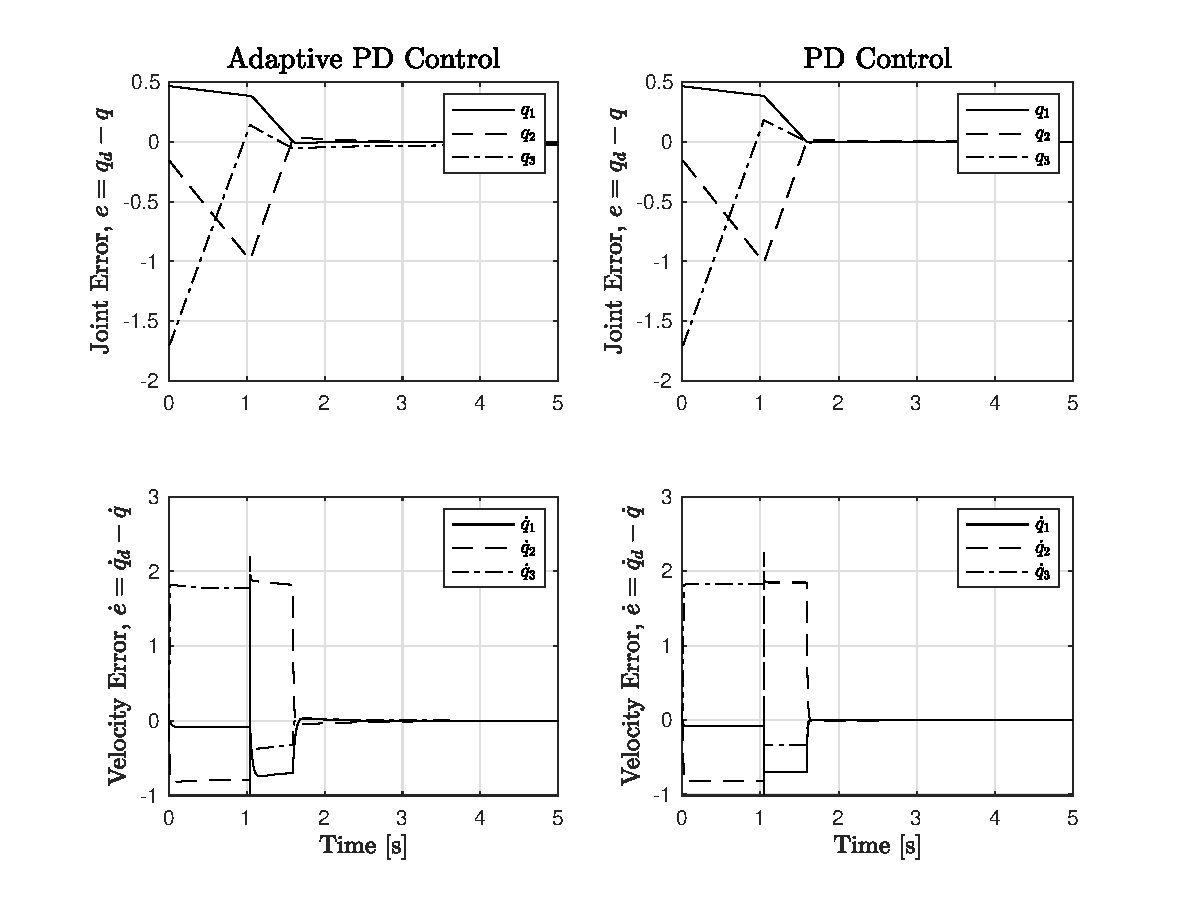
\includegraphics[width=0.7\textwidth]{figures/adpdErr.eps}
	\caption{Convergence of controller error dynamics}
	\label{fig:adpderr}
\end{figure}
As shown in Fig. \ref{fig:adpderr}, both controllers converge to the steady state value of zero in approximately the same time. One benefit to adaptive control however, is that as the mass changes (i.e. an object is picked up), the adaptation law accounts for the change in mass. With PD Control, there is no way to account for this mass addition and an increase in error is introduced.\\

We then evaluate each controller by it's ability to follow the desired trajectory provided by the $RRT^{*}$ path planning algorithm.
\begin{figure}[H]
	\centering
	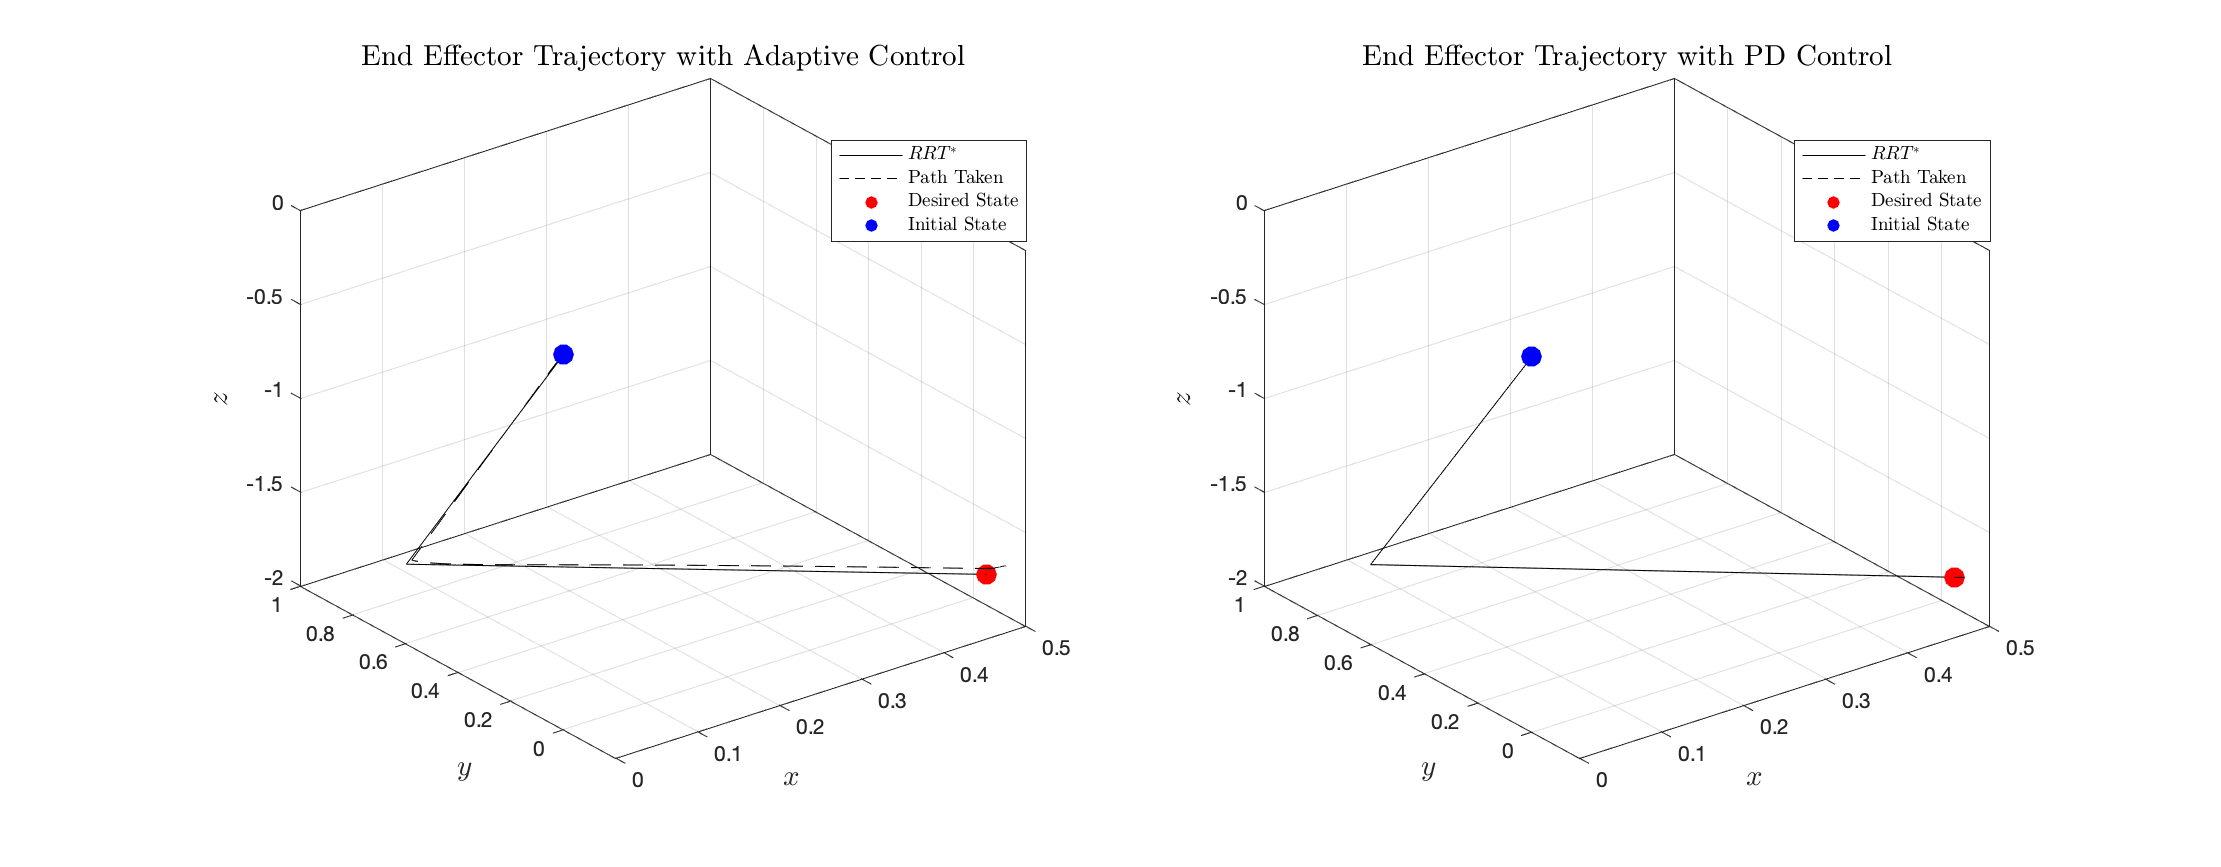
\includegraphics[width=0.9\textwidth]{figures/eeTraj.eps}
	\caption{Desired end-effector trajectory vs actual}
	\label{fig:eetraj}
\end{figure}
We can see from Fig. \ref{fig:eetraj} that in this case, the PD Controller maintains the desired trajectory more tightly than the Adaptive Control model. However, the error between the two control models is of an insignificant degree, thus the adaptive control model is chosen for the simulation.

	\section{Theory and Methods}
\section{Robotic Modeling}
\subsection{Approach}

The general equation of motion for a robotic manipulator can be expressed as:

\begin{equation}
  \label{eom-manipulator}
  M(q)\ddot{q} + C(q,\dot{q})\dot{q} + G(g) = \tau
\end{equation}

\noindent where $M(q)\in\mathbb{R}^{n\times n}$ is the mass matrix of the joints,
$C(q,\dot{q})\in\mathbb{R}^{n\times n}$ is the Coriolis matrix,
$G(q)\in\mathbb{R}^{n}$ is the conservative force vector acted on the arm by
gravity, and $\tau\in\mathbb{R}^{n}$ are the torques commanded to each joint.
Each of the terms on the left hand side of the equation can be directly modeled
when the manipulator joint information is known.
However, when this information is not available, a neural network can be used to
estimate the value of these matrices.

To model the conservative force vector, a robotic manipulator can be controlled
with a simple PD controller and brought to a stop at a given configuration value
$q$.
When the manipulator is at rest, Eq. (\ref{eom-manipulator}) simplifies to:

\begin{align}
  \label{eom-manipulator-stopped}
  M(q)*0 + C(q,0)*0 + G(q) &= \tau\\
  G(q) &= \tau
\end{align}

\noindent which allows the loss function for the function approximator
$\hat{G}(q)$ to be expressed as:

\begin{equation}
  \label{loss-function-gq}
  \hat{G}(q) - \tau = \delta_{Loss}
\end{equation}

To model the mass matrix with a function approximator $\hat{M}(q)$, we must
again model a loss function to train the network.
This proves more difficult, as the mass matrix must be isolated on the left hand
side of the equation.
However, if the number of acceleration samples taken at a given configuration
$q$ satisfy $rk(M(q)) = n_{samples}$, we could then construct an acceleration
matrix $\ddot{Q} = [\ddot{q_{1}}, \ddot{q_{2}}\dots\ddot{q_{n}}]$ which
satisfies $rk(\ddot{Q}) = rk(M(q)) = n$.
Properties of linear algebra now guarantee that a unique inverse of this matrix
must exist, and the equation can then be expressed as:

\begin{align}
  \label{eom-manipulator-accel}
  M(q)\ddot{Q} + C(q,\dot{Q})\dot{Q} + G(q) &= \tau\\
  \label{eom-manipulator-accel-m}
  M(q) &= \ddot{Q}^{-1}(\tau - G(q) - C(q,\dot{Q})\dot{Q})
\end{align}

The problem with this method is that the Coriolis term is still in place, and we
have no estimate for this value.
However, if we take our $\ddot{q}$ samples at the initial point when we first
begin accelerating, we should see that $\dot{q} \approx 0$, and thus Eq.
(\ref{eom-manipulator-accel-m}) can be expressed as:

\begin{align}
  M(q) = \ddot{Q}^{-1}(\tau - G(q))
\end{align}

\noindent which now allows for a loss function to be formulated.

For the Coriolis matrix, it directly depends on the mass matrix $M(q)$, and thus
once an estimate for $M(q)$ is formulated, the Coriolis matrix can be derived
from the given values of the $\hat{M}(q)$ matrix.

\subsection{Experiments}
The experiments for this section will include learning both $\hat{G}(q)$ and
$\hat{M}(q)$ using the proposed method above in two settings: One in a friction
free environment, and another when static friction is present.
The friction free case will be used primarily as a base case, and the accuracy
of both the $\hat{G}(q)$ and $\hat{M}(q)$ will be compared to their true values.
This will serve to see how effective this method is in general, as
friction begins complicating the process.

The frictional case will be further broken down into two sections.
The first will consist of learning the two maps without static friction
compensation, and the second will include static friction compensation.
Static friction will be modeled as a constant $\mu_{s}$, so this can easily be
added into the above formulations (primarily for the mass matrix case).

\section{Perception and Planning}
\subsection{Uncertainty in Configurations}
The robot configuration $q_1$, $q_2$, ..., $q_n$ determines how the robot will
interact with the task space and the end-effector.
Assuming that the end-effector has a camera on its end and can understand its
surroundings, the perception through said camera will be used to achieve motion
and interaction with an object in the task space.
A combination of the RRT path planning algorithm, Kalman filtering, and
Forward/Inverse kinematics will lead to the configuration that the robot is in
to have the end-effector reach the object.
An object with some mass $M_o$ will be placed in the task space.
The robot's purpose is to move to the object, pick it up, and move it to a
desired position.

\subsection{Approach}
The end-effector perception problem requires many disciplines of robotics.
First, a landmark based Kalman filter will be applied to the robot.
This will test our ability to move to the object.
Then, applying kinematic theory, the configuration of the robot to achieve the
end-effector location and orientation corresponding to the object will be
achieved.

\subsection*{Control Models}
To validate our control models, it is important to evaluate the error dynamics associated with the controllers. To do this, we begin with the comparison of the error convergence between the Adaptive Control model and the classical PD Control model. This comparison was made with a fixed, known weight, as well as no noise in the joint values.
\begin{figure}[H]
	\centering
	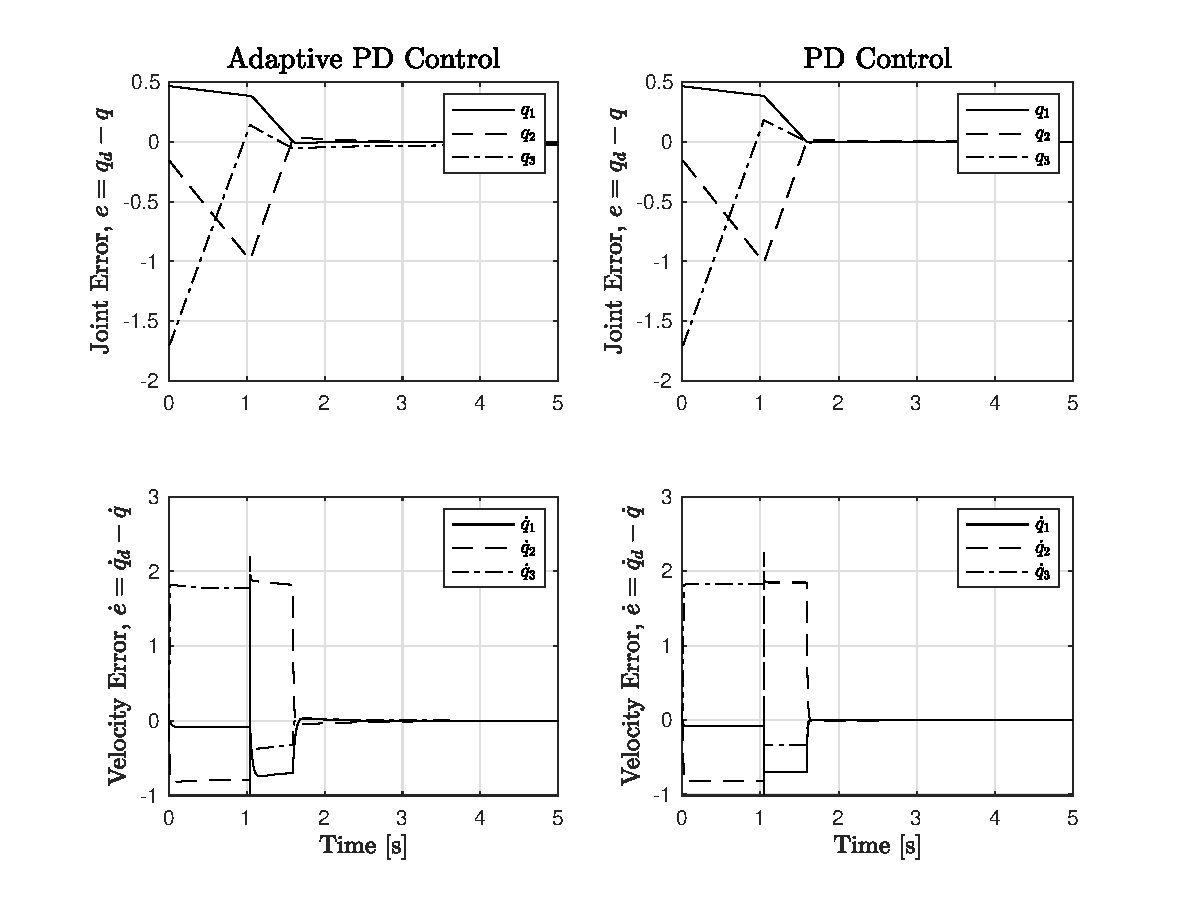
\includegraphics[width=0.7\textwidth]{figures/adpdErr.eps}
	\caption{Convergence of controller error dynamics}
	\label{fig:adpderr}
\end{figure}
As shown in Fig. \ref{fig:adpderr}, both controllers converge to the steady state value of zero in approximately the same time. One benefit to adaptive control however, is that as the mass changes (i.e. an object is picked up), the adaptation law accounts for the change in mass. With PD Control, there is no way to account for this mass addition and an increase in error is introduced.\\

We then evaluate each controller by it's ability to follow the desired trajectory provided by the $RRT^{*}$ path planning algorithm.
\begin{figure}[H]
	\centering
	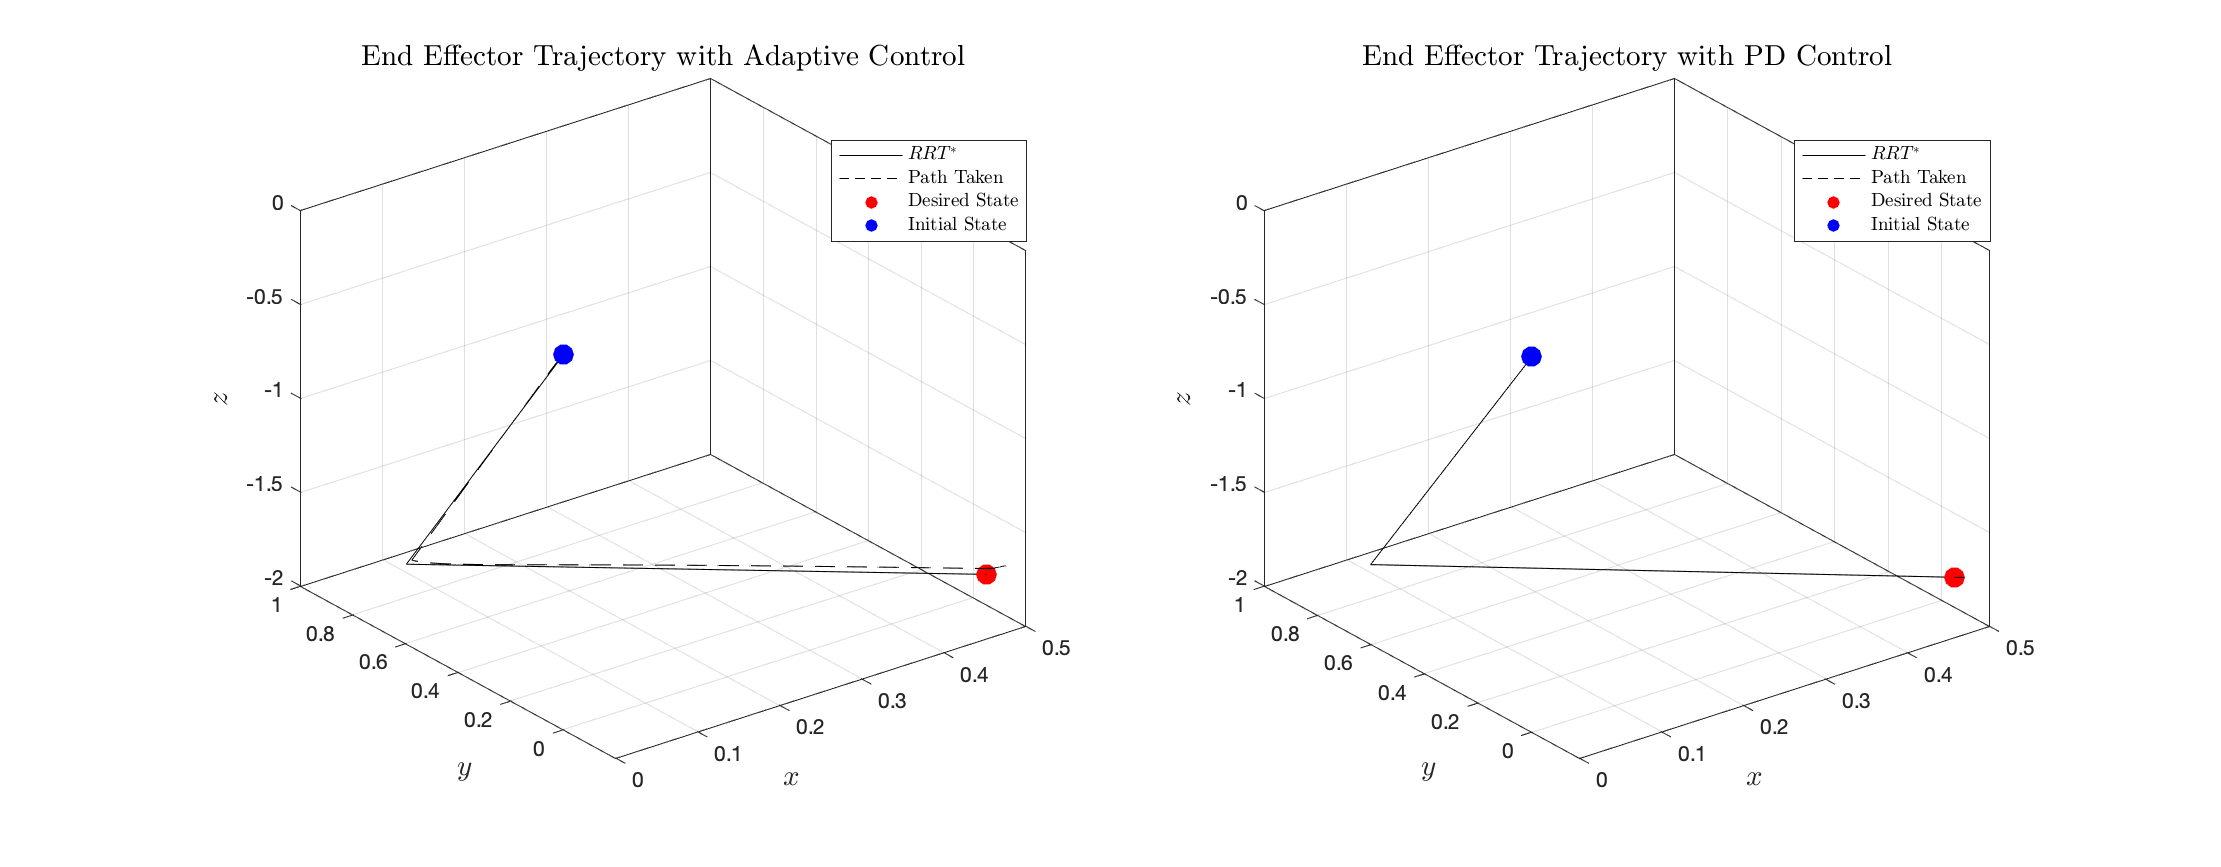
\includegraphics[width=0.9\textwidth]{figures/eeTraj.eps}
	\caption{Desired end-effector trajectory vs actual}
	\label{fig:eetraj}
\end{figure}
We can see from Fig. \ref{fig:eetraj} that in this case, the PD Controller maintains the desired trajectory more tightly than the Adaptive Control model. However, the error between the two control models is of an insignificant degree, thus the adaptive control model is chosen for the simulation.


	\section{Experiments}
One primary experiment was run to test the effectiveness of the mass neural network, the adaptive controller, and the Kalman filter.
This was the task proposed in the introduction, consisting of three phases.
Each of these phases provided different data to be collected and measured to see how well each method performed.
In addition, the loss metrics of the mass neural network during training will be plotted and discussed.

\subsection*{Controls Experiment}
Both the adaptive control and the mass matrix neural network control were tested against each other in the three different phases.
These phases consisted of the initial trajectory towards the target object, moving the object of unknown mass to the goal state, and finally returning to the original position the arm started in.
Both of these methods were compared to a baseline of a standard PD trajectory tracking controller as well, to serve as a baseline for performance.
The metric for these experiments was the error in tracked trajectory for both joint configurations and velocities under control.

\subsection*{Mass Experiment}
The adaptive control was also tested multiple times in the second phase (moving the object of unknown mass) where the mass was varied.
The performance under differing weights was of particular interest.
The metric for this experiment was the error in tracked trajectory for the three joint configurations and velocities during the control.

\subsection*{Kalman Filter Experiment}
To measure the effectiveness of the Kalman filter, both the stationary and moving filter results were examined.
The error in actual position (known due to simulation) versus predicted position was used as the metric.
If effectively implemented, the error in predicted position should begin to converge towards the actual position as more samples are acquired and the confidence of the filter increases.

The experiments will use white noise samples from the Gaussian distribution $n\sim \mathcal{N}(0,0.1)$.
This variance provides enough noise to show the filter working effectively, but not so much that it cannot provide accurate estimates within the short time span of the trajectory.

\subsection*{Control Models}
To validate our control models, it is important to evaluate the error dynamics associated with the controllers. To do this, we begin with the comparison of the error convergence between the Adaptive Control model and the classical PD Control model. This comparison was made with a fixed, known weight, as well as no noise in the joint values.
\begin{figure}[H]
	\centering
	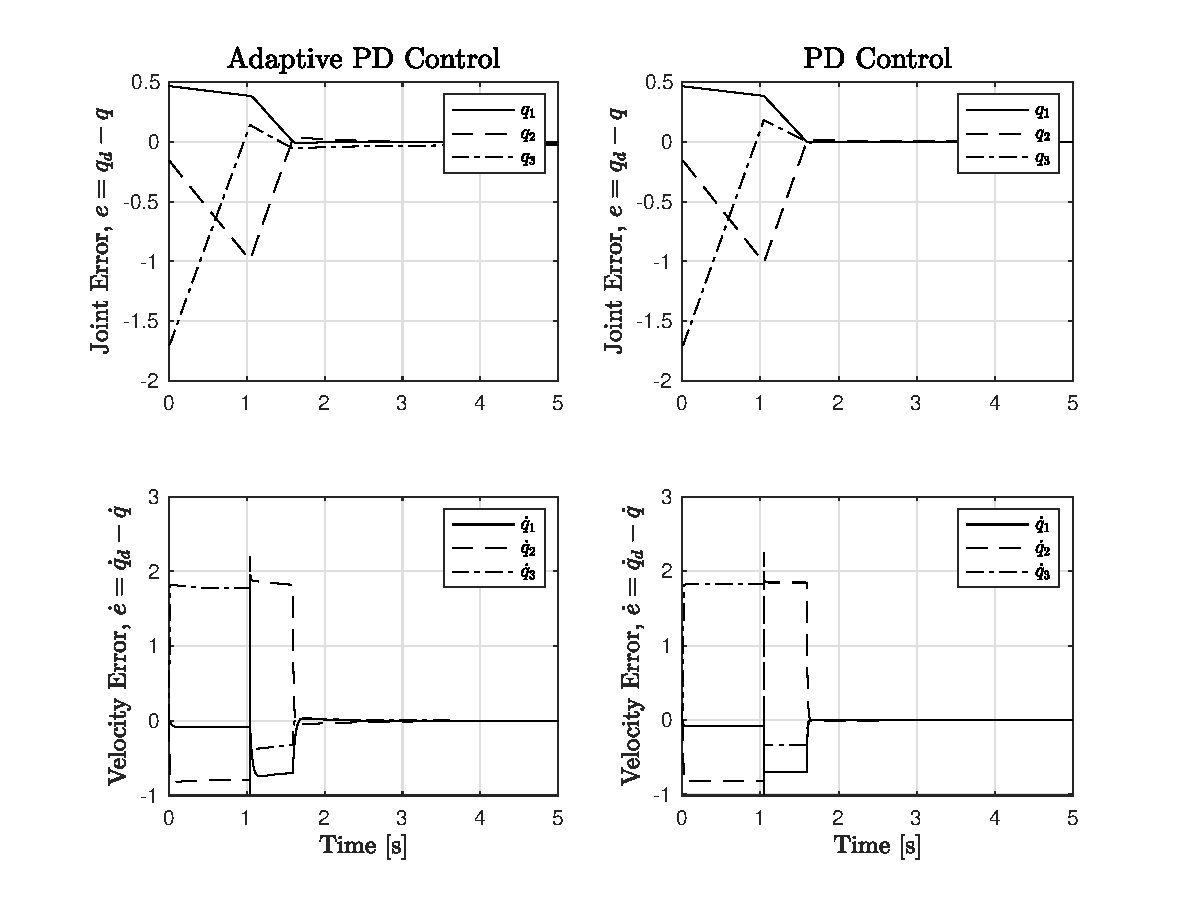
\includegraphics[width=0.7\textwidth]{figures/adpdErr.eps}
	\caption{Convergence of controller error dynamics}
	\label{fig:adpderr}
\end{figure}
As shown in Fig. \ref{fig:adpderr}, both controllers converge to the steady state value of zero in approximately the same time. One benefit to adaptive control however, is that as the mass changes (i.e. an object is picked up), the adaptation law accounts for the change in mass. With PD Control, there is no way to account for this mass addition and an increase in error is introduced.\\

We then evaluate each controller by it's ability to follow the desired trajectory provided by the $RRT^{*}$ path planning algorithm.
\begin{figure}[H]
	\centering
	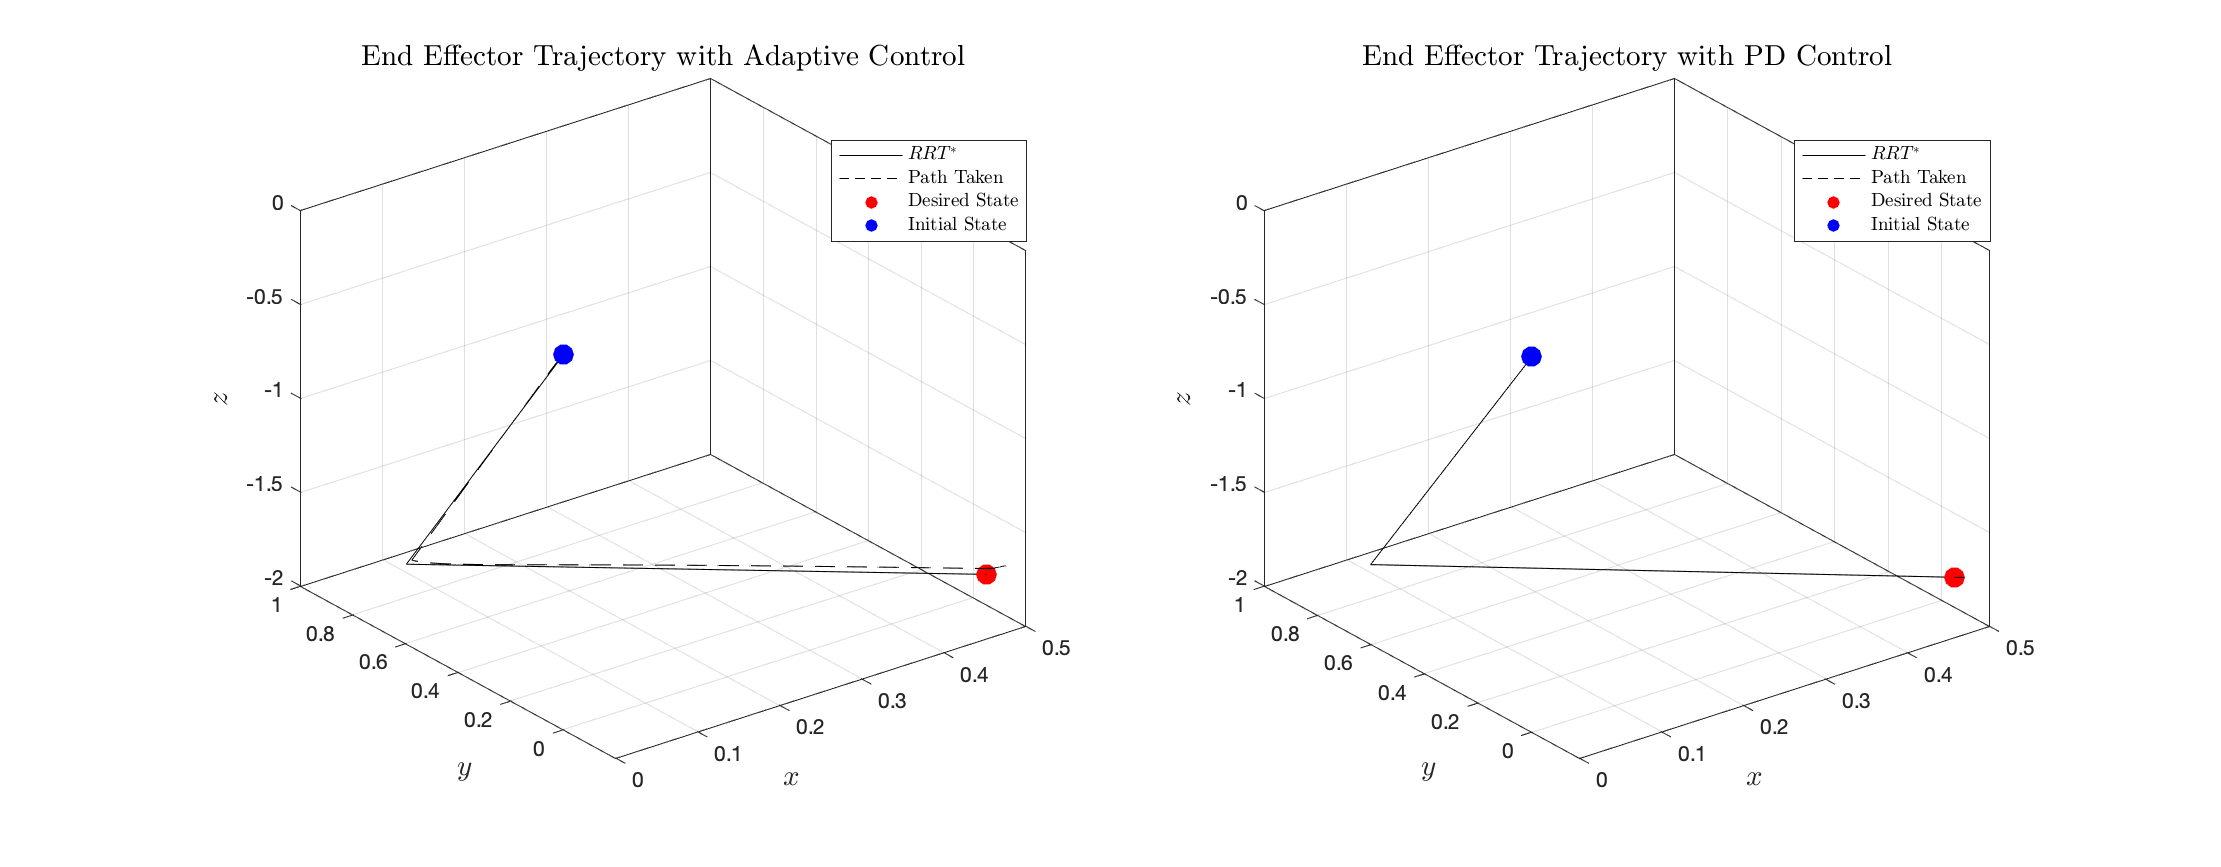
\includegraphics[width=0.9\textwidth]{figures/eeTraj.eps}
	\caption{Desired end-effector trajectory vs actual}
	\label{fig:eetraj}
\end{figure}
We can see from Fig. \ref{fig:eetraj} that in this case, the PD Controller maintains the desired trajectory more tightly than the Adaptive Control model. However, the error between the two control models is of an insignificant degree, thus the adaptive control model is chosen for the simulation.


	\section{Results}
%\section{Robotic Modeling}
\subsection{Approach}

The general equation of motion for a robotic manipulator can be expressed as:

\begin{equation}
  \label{eom-manipulator}
  M(q)\ddot{q} + C(q,\dot{q})\dot{q} + G(g) = \tau
\end{equation}

\noindent where $M(q)\in\mathbb{R}^{n\times n}$ is the mass matrix of the joints,
$C(q,\dot{q})\in\mathbb{R}^{n\times n}$ is the Coriolis matrix,
$G(q)\in\mathbb{R}^{n}$ is the conservative force vector acted on the arm by
gravity, and $\tau\in\mathbb{R}^{n}$ are the torques commanded to each joint.
Each of the terms on the left hand side of the equation can be directly modeled
when the manipulator joint information is known.
However, when this information is not available, a neural network can be used to
estimate the value of these matrices.

To model the conservative force vector, a robotic manipulator can be controlled
with a simple PD controller and brought to a stop at a given configuration value
$q$.
When the manipulator is at rest, Eq. (\ref{eom-manipulator}) simplifies to:

\begin{align}
  \label{eom-manipulator-stopped}
  M(q)*0 + C(q,0)*0 + G(q) &= \tau\\
  G(q) &= \tau
\end{align}

\noindent which allows the loss function for the function approximator
$\hat{G}(q)$ to be expressed as:

\begin{equation}
  \label{loss-function-gq}
  \hat{G}(q) - \tau = \delta_{Loss}
\end{equation}

To model the mass matrix with a function approximator $\hat{M}(q)$, we must
again model a loss function to train the network.
This proves more difficult, as the mass matrix must be isolated on the left hand
side of the equation.
However, if the number of acceleration samples taken at a given configuration
$q$ satisfy $rk(M(q)) = n_{samples}$, we could then construct an acceleration
matrix $\ddot{Q} = [\ddot{q_{1}}, \ddot{q_{2}}\dots\ddot{q_{n}}]$ which
satisfies $rk(\ddot{Q}) = rk(M(q)) = n$.
Properties of linear algebra now guarantee that a unique inverse of this matrix
must exist, and the equation can then be expressed as:

\begin{align}
  \label{eom-manipulator-accel}
  M(q)\ddot{Q} + C(q,\dot{Q})\dot{Q} + G(q) &= \tau\\
  \label{eom-manipulator-accel-m}
  M(q) &= \ddot{Q}^{-1}(\tau - G(q) - C(q,\dot{Q})\dot{Q})
\end{align}

The problem with this method is that the Coriolis term is still in place, and we
have no estimate for this value.
However, if we take our $\ddot{q}$ samples at the initial point when we first
begin accelerating, we should see that $\dot{q} \approx 0$, and thus Eq.
(\ref{eom-manipulator-accel-m}) can be expressed as:

\begin{align}
  M(q) = \ddot{Q}^{-1}(\tau - G(q))
\end{align}

\noindent which now allows for a loss function to be formulated.

For the Coriolis matrix, it directly depends on the mass matrix $M(q)$, and thus
once an estimate for $M(q)$ is formulated, the Coriolis matrix can be derived
from the given values of the $\hat{M}(q)$ matrix.

\subsection{Experiments}
The experiments for this section will include learning both $\hat{G}(q)$ and
$\hat{M}(q)$ using the proposed method above in two settings: One in a friction
free environment, and another when static friction is present.
The friction free case will be used primarily as a base case, and the accuracy
of both the $\hat{G}(q)$ and $\hat{M}(q)$ will be compared to their true values.
This will serve to see how effective this method is in general, as
friction begins complicating the process.

The frictional case will be further broken down into two sections.
The first will consist of learning the two maps without static friction
compensation, and the second will include static friction compensation.
Static friction will be modeled as a constant $\mu_{s}$, so this can easily be
added into the above formulations (primarily for the mass matrix case).

%\section{Perception and Planning}
\subsection{Uncertainty in Configurations}
The robot configuration $q_1$, $q_2$, ..., $q_n$ determines how the robot will
interact with the task space and the end-effector.
Assuming that the end-effector has a camera on its end and can understand its
surroundings, the perception through said camera will be used to achieve motion
and interaction with an object in the task space.
A combination of the RRT path planning algorithm, Kalman filtering, and
Forward/Inverse kinematics will lead to the configuration that the robot is in
to have the end-effector reach the object.
An object with some mass $M_o$ will be placed in the task space.
The robot's purpose is to move to the object, pick it up, and move it to a
desired position.

\subsection{Approach}
The end-effector perception problem requires many disciplines of robotics.
First, a landmark based Kalman filter will be applied to the robot.
This will test our ability to move to the object.
Then, applying kinematic theory, the configuration of the robot to achieve the
end-effector location and orientation corresponding to the object will be
achieved.

%\subsection*{Control Models}
To validate our control models, it is important to evaluate the error dynamics associated with the controllers. To do this, we begin with the comparison of the error convergence between the Adaptive Control model and the classical PD Control model. This comparison was made with a fixed, known weight, as well as no noise in the joint values.
\begin{figure}[H]
	\centering
	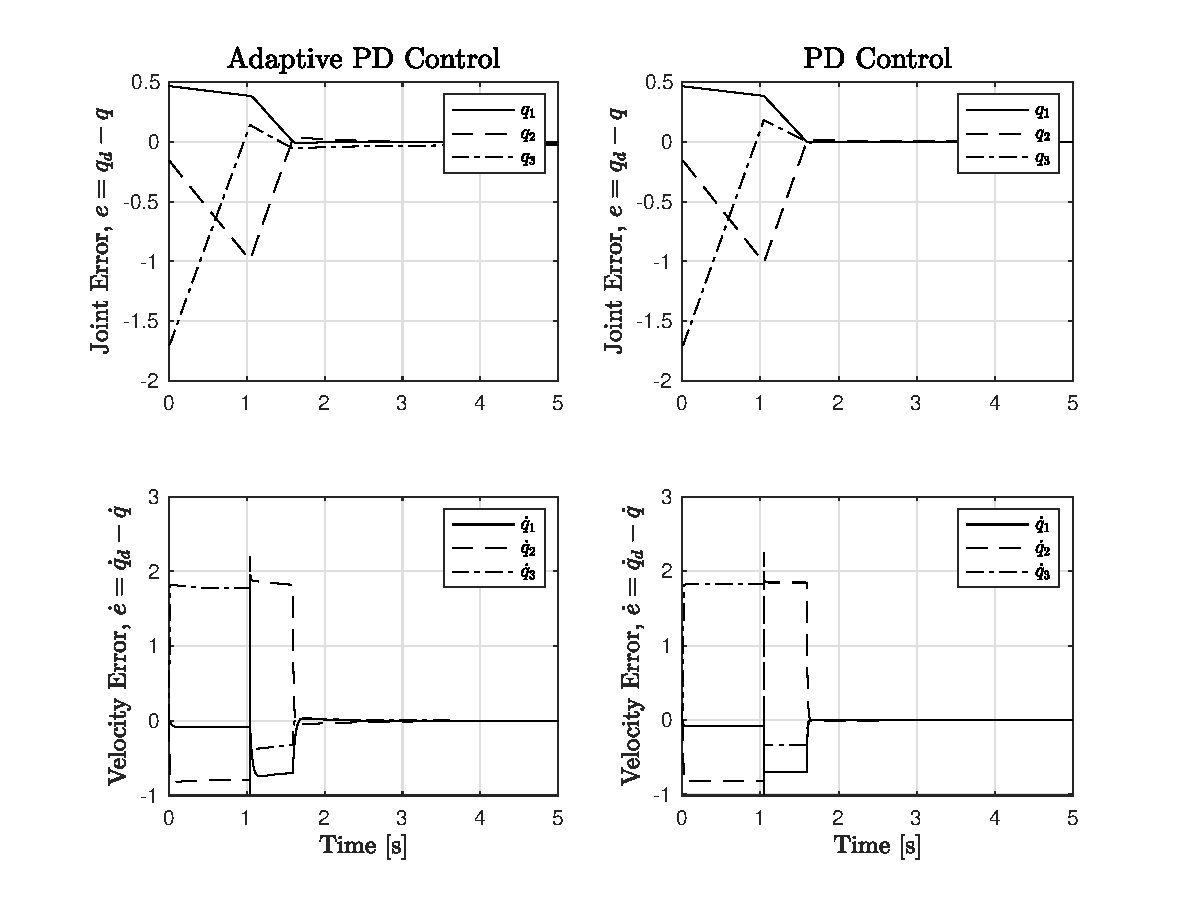
\includegraphics[width=0.7\textwidth]{figures/adpdErr.eps}
	\caption{Convergence of controller error dynamics}
	\label{fig:adpderr}
\end{figure}
As shown in Fig. \ref{fig:adpderr}, both controllers converge to the steady state value of zero in approximately the same time. One benefit to adaptive control however, is that as the mass changes (i.e. an object is picked up), the adaptation law accounts for the change in mass. With PD Control, there is no way to account for this mass addition and an increase in error is introduced.\\

We then evaluate each controller by it's ability to follow the desired trajectory provided by the $RRT^{*}$ path planning algorithm.
\begin{figure}[H]
	\centering
	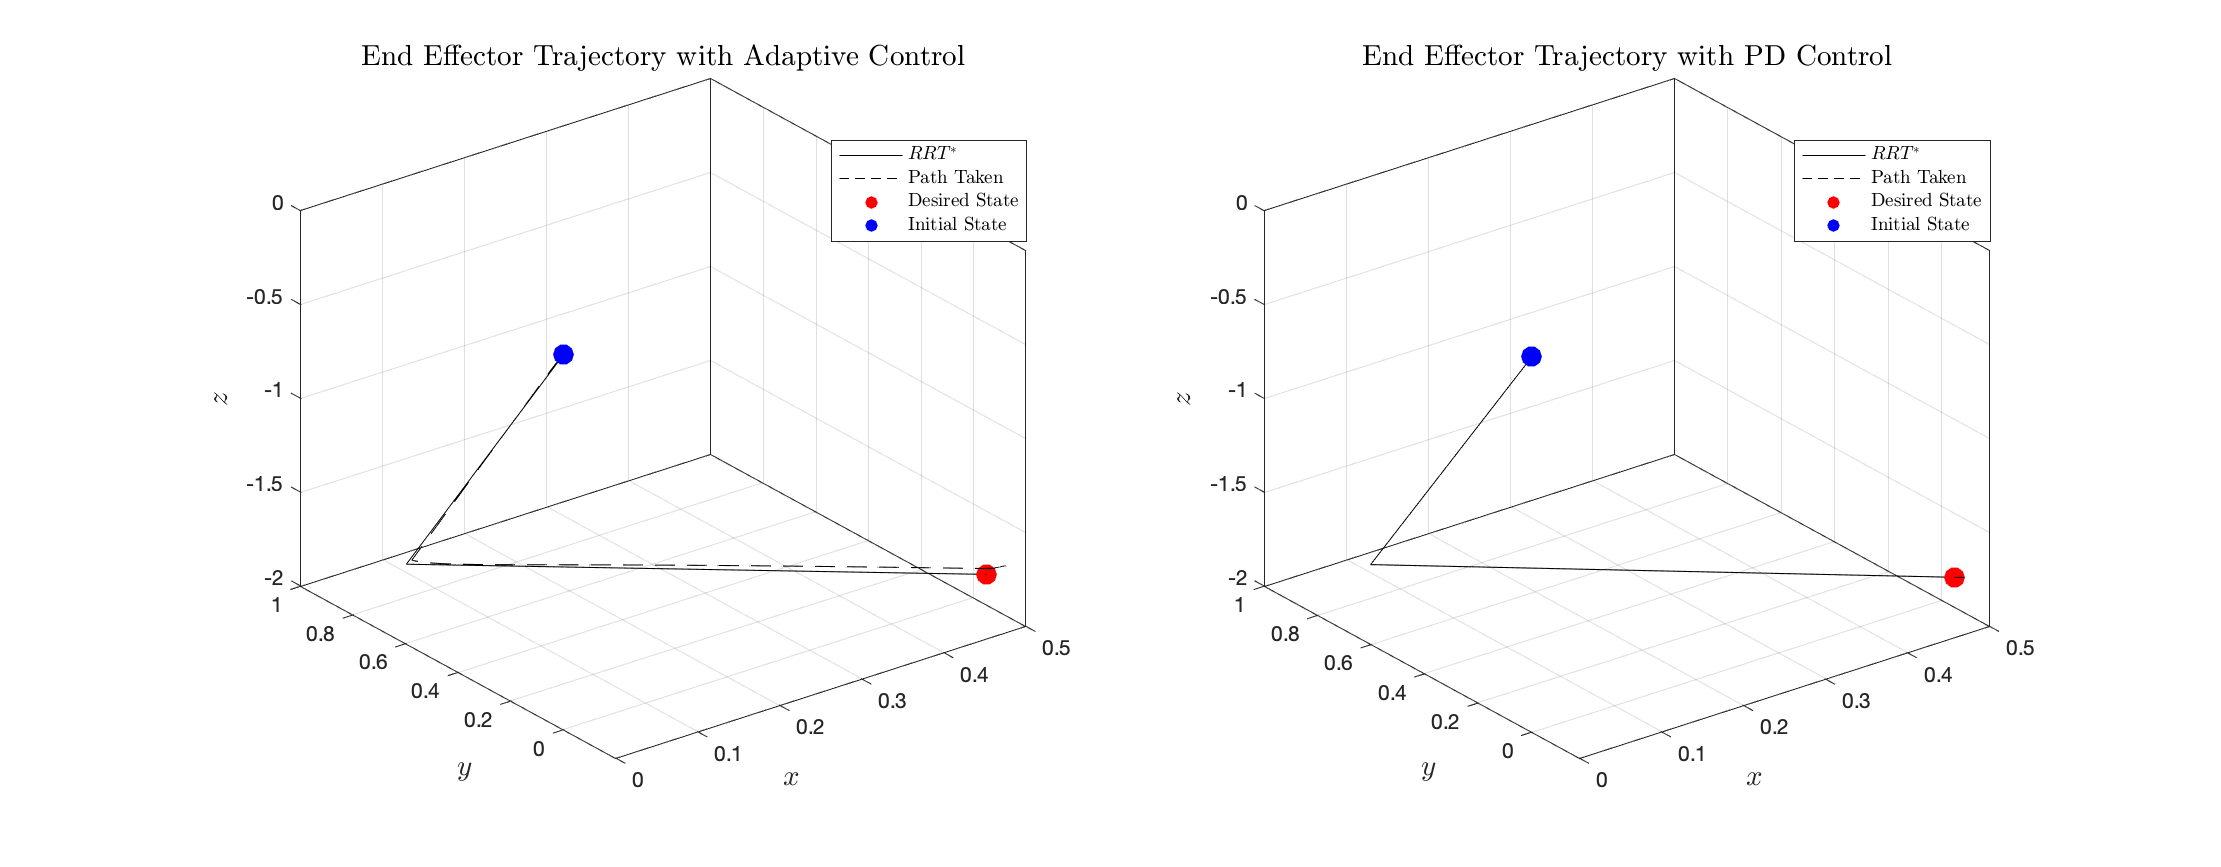
\includegraphics[width=0.9\textwidth]{figures/eeTraj.eps}
	\caption{Desired end-effector trajectory vs actual}
	\label{fig:eetraj}
\end{figure}
We can see from Fig. \ref{fig:eetraj} that in this case, the PD Controller maintains the desired trajectory more tightly than the Adaptive Control model. However, the error between the two control models is of an insignificant degree, thus the adaptive control model is chosen for the simulation.

	\section{Conclusion}
%\section{Robotic Modeling}
\subsection{Approach}

The general equation of motion for a robotic manipulator can be expressed as:

\begin{equation}
  \label{eom-manipulator}
  M(q)\ddot{q} + C(q,\dot{q})\dot{q} + G(g) = \tau
\end{equation}

\noindent where $M(q)\in\mathbb{R}^{n\times n}$ is the mass matrix of the joints,
$C(q,\dot{q})\in\mathbb{R}^{n\times n}$ is the Coriolis matrix,
$G(q)\in\mathbb{R}^{n}$ is the conservative force vector acted on the arm by
gravity, and $\tau\in\mathbb{R}^{n}$ are the torques commanded to each joint.
Each of the terms on the left hand side of the equation can be directly modeled
when the manipulator joint information is known.
However, when this information is not available, a neural network can be used to
estimate the value of these matrices.

To model the conservative force vector, a robotic manipulator can be controlled
with a simple PD controller and brought to a stop at a given configuration value
$q$.
When the manipulator is at rest, Eq. (\ref{eom-manipulator}) simplifies to:

\begin{align}
  \label{eom-manipulator-stopped}
  M(q)*0 + C(q,0)*0 + G(q) &= \tau\\
  G(q) &= \tau
\end{align}

\noindent which allows the loss function for the function approximator
$\hat{G}(q)$ to be expressed as:

\begin{equation}
  \label{loss-function-gq}
  \hat{G}(q) - \tau = \delta_{Loss}
\end{equation}

To model the mass matrix with a function approximator $\hat{M}(q)$, we must
again model a loss function to train the network.
This proves more difficult, as the mass matrix must be isolated on the left hand
side of the equation.
However, if the number of acceleration samples taken at a given configuration
$q$ satisfy $rk(M(q)) = n_{samples}$, we could then construct an acceleration
matrix $\ddot{Q} = [\ddot{q_{1}}, \ddot{q_{2}}\dots\ddot{q_{n}}]$ which
satisfies $rk(\ddot{Q}) = rk(M(q)) = n$.
Properties of linear algebra now guarantee that a unique inverse of this matrix
must exist, and the equation can then be expressed as:

\begin{align}
  \label{eom-manipulator-accel}
  M(q)\ddot{Q} + C(q,\dot{Q})\dot{Q} + G(q) &= \tau\\
  \label{eom-manipulator-accel-m}
  M(q) &= \ddot{Q}^{-1}(\tau - G(q) - C(q,\dot{Q})\dot{Q})
\end{align}

The problem with this method is that the Coriolis term is still in place, and we
have no estimate for this value.
However, if we take our $\ddot{q}$ samples at the initial point when we first
begin accelerating, we should see that $\dot{q} \approx 0$, and thus Eq.
(\ref{eom-manipulator-accel-m}) can be expressed as:

\begin{align}
  M(q) = \ddot{Q}^{-1}(\tau - G(q))
\end{align}

\noindent which now allows for a loss function to be formulated.

For the Coriolis matrix, it directly depends on the mass matrix $M(q)$, and thus
once an estimate for $M(q)$ is formulated, the Coriolis matrix can be derived
from the given values of the $\hat{M}(q)$ matrix.

\subsection{Experiments}
The experiments for this section will include learning both $\hat{G}(q)$ and
$\hat{M}(q)$ using the proposed method above in two settings: One in a friction
free environment, and another when static friction is present.
The friction free case will be used primarily as a base case, and the accuracy
of both the $\hat{G}(q)$ and $\hat{M}(q)$ will be compared to their true values.
This will serve to see how effective this method is in general, as
friction begins complicating the process.

The frictional case will be further broken down into two sections.
The first will consist of learning the two maps without static friction
compensation, and the second will include static friction compensation.
Static friction will be modeled as a constant $\mu_{s}$, so this can easily be
added into the above formulations (primarily for the mass matrix case).

%\section{Perception and Planning}
\subsection{Uncertainty in Configurations}
The robot configuration $q_1$, $q_2$, ..., $q_n$ determines how the robot will
interact with the task space and the end-effector.
Assuming that the end-effector has a camera on its end and can understand its
surroundings, the perception through said camera will be used to achieve motion
and interaction with an object in the task space.
A combination of the RRT path planning algorithm, Kalman filtering, and
Forward/Inverse kinematics will lead to the configuration that the robot is in
to have the end-effector reach the object.
An object with some mass $M_o$ will be placed in the task space.
The robot's purpose is to move to the object, pick it up, and move it to a
desired position.

\subsection{Approach}
The end-effector perception problem requires many disciplines of robotics.
First, a landmark based Kalman filter will be applied to the robot.
This will test our ability to move to the object.
Then, applying kinematic theory, the configuration of the robot to achieve the
end-effector location and orientation corresponding to the object will be
achieved.

\subsection*{Control Models}
To validate our control models, it is important to evaluate the error dynamics associated with the controllers. To do this, we begin with the comparison of the error convergence between the Adaptive Control model and the classical PD Control model. This comparison was made with a fixed, known weight, as well as no noise in the joint values.
\begin{figure}[H]
	\centering
	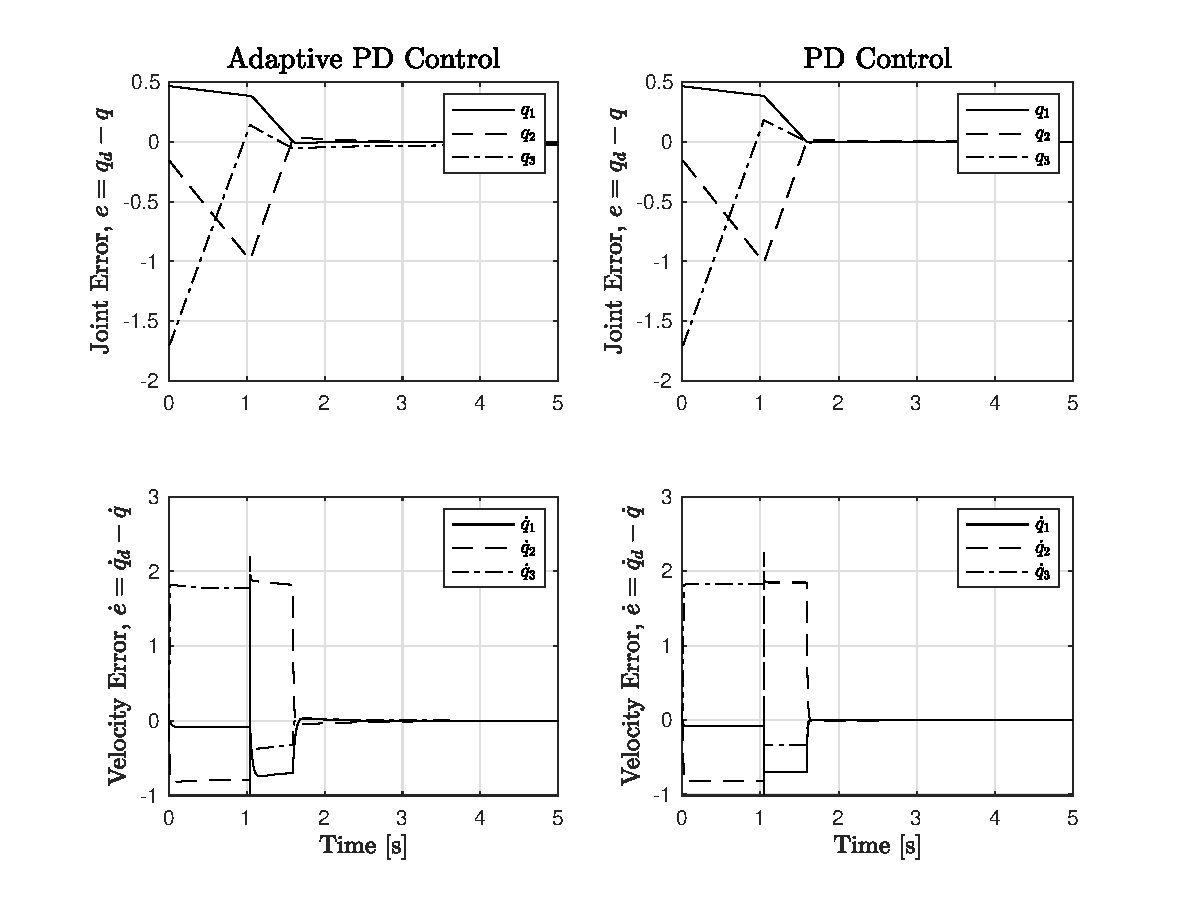
\includegraphics[width=0.7\textwidth]{figures/adpdErr.eps}
	\caption{Convergence of controller error dynamics}
	\label{fig:adpderr}
\end{figure}
As shown in Fig. \ref{fig:adpderr}, both controllers converge to the steady state value of zero in approximately the same time. One benefit to adaptive control however, is that as the mass changes (i.e. an object is picked up), the adaptation law accounts for the change in mass. With PD Control, there is no way to account for this mass addition and an increase in error is introduced.\\

We then evaluate each controller by it's ability to follow the desired trajectory provided by the $RRT^{*}$ path planning algorithm.
\begin{figure}[H]
	\centering
	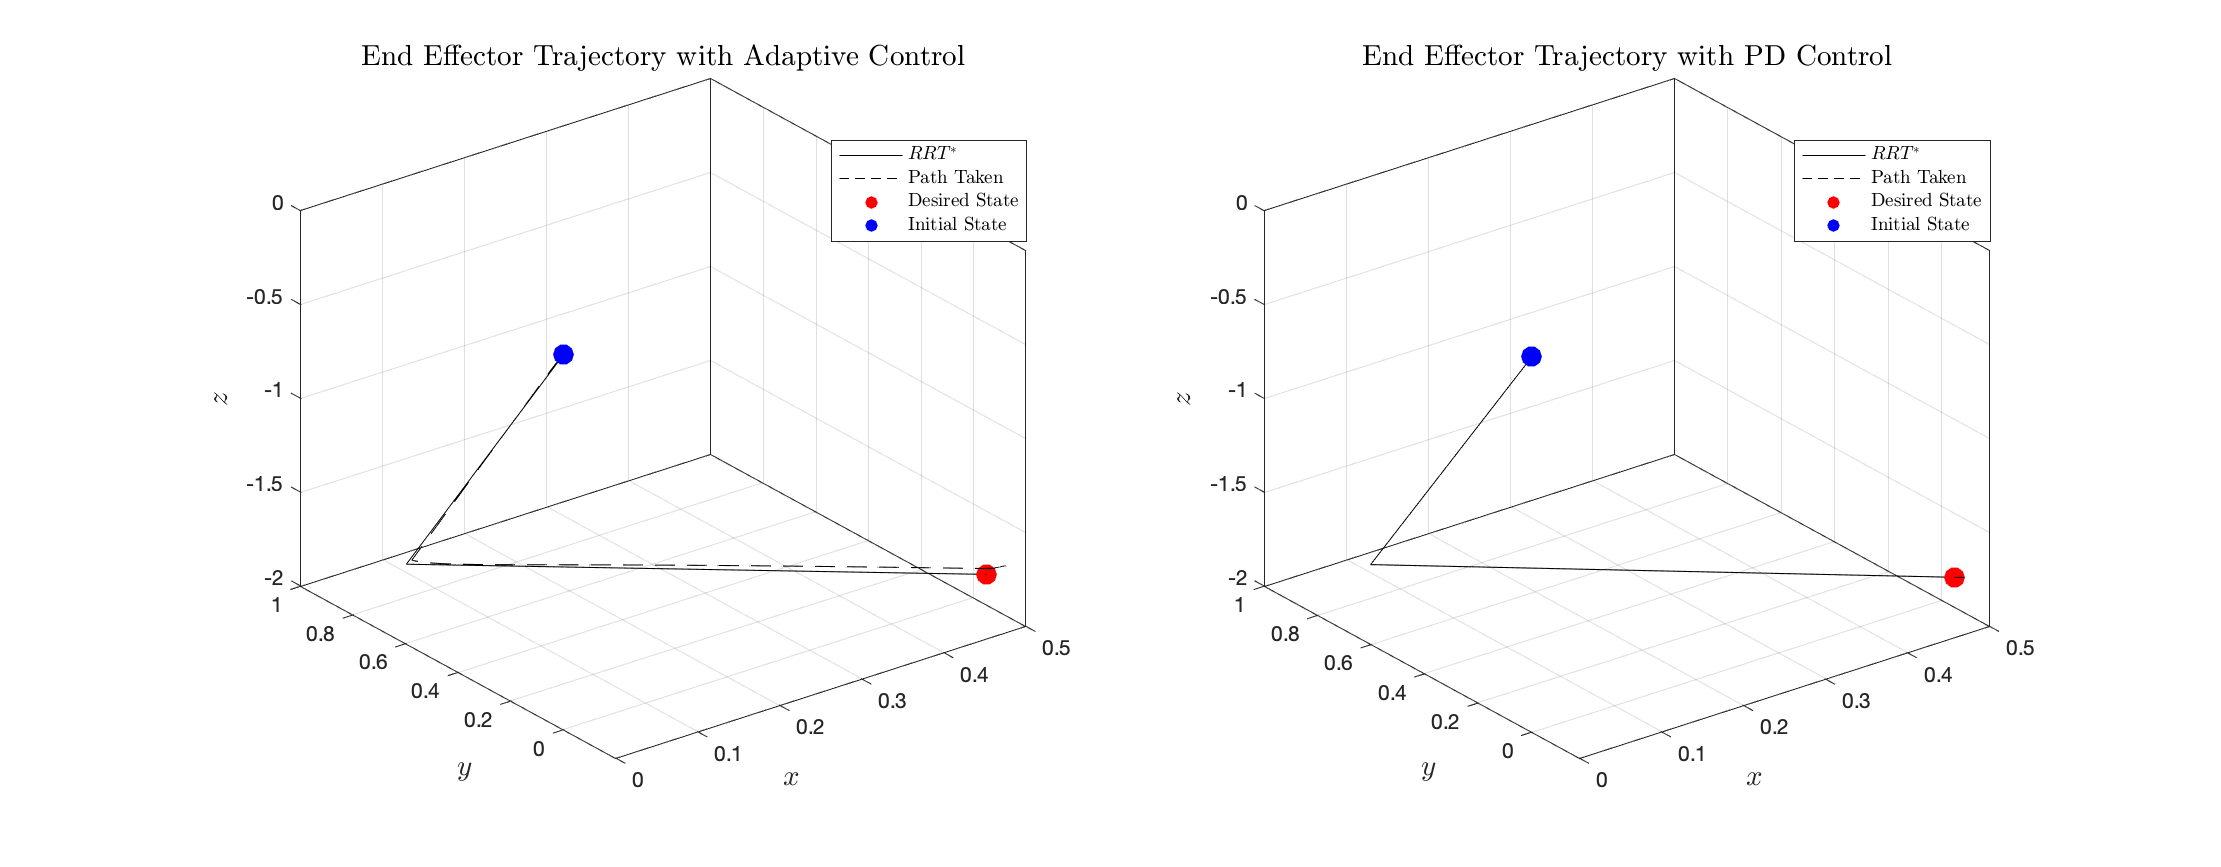
\includegraphics[width=0.9\textwidth]{figures/eeTraj.eps}
	\caption{Desired end-effector trajectory vs actual}
	\label{fig:eetraj}
\end{figure}
We can see from Fig. \ref{fig:eetraj} that in this case, the PD Controller maintains the desired trajectory more tightly than the Adaptive Control model. However, the error between the two control models is of an insignificant degree, thus the adaptive control model is chosen for the simulation.
 %Actually the conclusion
	
	\newpage
	\printbibliography[heading=bibintoc,title=Works Cited]

\end{document}
